\documentclass[a4paper,12pt]{article}
\newcommand{\cc}[1]{\multicolumn{1}{c}{#1}}
\newcommand{\m}[1]{\mathbf #1}
\newcommand{\wh}{\widehat}
\newcommand{\bra}[1]{\langle #1|}
\newcommand{\ket}[1]{|#1\rangle }
\usepackage{molsoc}
\usepackage{longtable}
\usepackage{wrapfig}
\usepackage{amsmath,amsthm}
\def\thismanual{MolSOC}
\def\molsocauthor{Sandro Giuseppe Chiodo}
\newif\ifprintauthor\printauthorfalse
\def\variable#1{{\keyfont #1}}
\makeindex
%
\begin{document}
\def\thismanual{User's Manual}
\begin{titlepage}
\begin{center}
\hrule depth 1pt height 1pt
\vskip 5mm
{\huge {\sf MolSOC} version 0.1}
\vskip 5mm
{\LARGE \thismanual}
\vskip 5mm
\hrule depth 1pt height 1pt
\vskip 0pt plus 1 fil
\vskip 5mm
\centerline{\logo[80mm]}
\vskip 5mm
\vskip 0pt plus 2 fil
\hrule depth 1pt height 1pt
\vskip 10mm
{\noindent\raise1ex\hbox{\normalsize} {\bf Author: Sandro Giuseppe Chiodo}}
\end{center}
\end{titlepage}
\newpage
\section{Introduction}

The basic theoretical approach implemented in {\sf MolSOC} provides a procedure that 
takes explicitly into account 
monodeterminantal wave functions of a pair of pre-optimized states, coupled through 
a Spin-Orbit Coupling (SOC) operator. More explicitly, a full Breit-Pauli operator\cite{Breit}, 
\begin{equation}
\begin{split}
 \wh H^{SO}_{BP} = & \frac {e^2} {2m^2_e c^2} \sum_{i=1}^{N_{el}} \biggl{\{} \sum_{\alpha = 1}^{N_{A}}
 Z_{\alpha} \biggl{(} \frac {\m{r}_{i \alpha}} {r_{i \alpha} ^3} \times
\m{p}_{i} \biggl{)} \cdot \m{s}_{i} \\
 & - \sum_{j \ne i}^{N_{el}} \biggl{(} \frac {\m{r}_{ij}} {r^3_{ij}} \times \m{p}_{i} \biggl{)}
\cdot (\m{s}_{i} + 2\m{s}_{j}) \biggl{\}}, \label{1}
\end{split}
\end{equation}
and a reduced screened-nuclear charge one,
\begin{equation}
 \wh H_{SO} = \frac {e^2} {2m^2_e c^2} \sum_{i=1}^{N_{el}} \sum_{\alpha = 1}^{N_{A}}
 Z_{eff}(\alpha) \biggl{(} \frac {\m{r}_{i \alpha}} {r_{i \alpha} ^3} \times
\m{p}_{i} \biggl{)} \cdot \m{s}_{i}, \label{1}
\end{equation}
are considered.
The explicit expressions of the derived matrix elements 
and more informations about this method can be found in earlier detailed 
works\cite{Chiod1,Chiod2}.

To run {\sf MolSOC} are needed the Self-Consistent Field (SCF) Molecular Orbitals (MO) 
linear combination coefficients of the two states which, in principle, 
can be supplied by means of many quantum mechanical codes. However, the present version can support only
formatted checkpoint files of the {\sf GAUSSIAN 03} program package, the formatted {\em mos} files
of the {\sf TURBOMOLE V6.0} code, and the unformatted {\em deMon.rst} files of the
{\sf deMon V1.02} code. \\ 
The sets of MOs, due 
to the separate optimization of the two states, can be not quite orthogonal to each other. 
To make these MOs pairwise orthogonals, biorthogonalization is 
performed by using transformation matrices, which, in turns, are 
obtained by Singular Value Decomposition (SVD) of the two-state MO overlap matrix.

Notice that the most tedious work is in the preliminary procedure for preparing MOs of the two states.
We strongly recommend to pay close attention to this procedure, to look at the MOs of the two states, 
to compare them before to be coupled. 
One can be interested to specific MO configurations, even belonging to excited states. It is not 
instantly obvious that, sometime, these are not properly preserved during the SCF iterations. However, 
one can refine particular strategies to avoid this drawback\cite{Chiod1,Chiod2}, 
or one can easily find with {\sf GAUSSIAN 03} typical therapeutic keywords fit for this purpose, like the 
{\em symm} keyword.

\section{{\sf MolSOC} installation}
\subsection{{\sf MolSOC} installation}
To compile {\sf MolSOC} is very simple, just you need to open the {\bf Makefile}, located in the
source code directory ({\bf source}), and uncomment the lines where are defined 
own fortran compiler, flags, and linker. Note that {\sf MolSOC} is supplied with LAPACK and 
BLAS math libraries which must be compiled before the source code. The math library {\bf Makefile}
is located in the {\bf lib} directory. These {\bf Makefiles} contain the targets specific 
to the following compilers:
\begin{enumerate}
\renewcommand{\labelenumi}{(\roman{enumi})}
\item OSF/1 Tru64 compiler;
\item Intel Fortran compiler;
\item Portland Group Fortran-90 compiler.
\end{enumerate}

{\sf MolSOC} needs a working Fortran 90 compiler. The 
following installation procedure can be used:
\begin{enumerate}
\item Unpack the {\sf MolSOC} distribution files in subdirectory {\bf molsoc0.1} of own desired directory;
\item Go to the {\bf molsoc0.1/lib} subdirectory and uncomment or add own fortran compiler, flags, and linker in the {\bf Makefile};
\item Issue in this subdirectory the command {\bf make} to compile the {\sf MolSOC} libreries;
\item Go to the {\bf molsoc0.1/source} subdirectory and uncomment or add own fortran compiler, flags, and linker in the {\bf Makefile};
\item Issue in this subdirectory the command {\bf make} to compile the {\sf MolSOC} source code. The {\bf molsoc0.1.exe} executable will be created and placed in the directory {\bf molsoc0.1/bin};
\item To make the {\sf MolSOC} executable permanently recognizable by the operating system 
by simply typing {\bf molsoc0.1.exe} from the linux shell prompt, add its location path to 
own shell initialization file ({\bf .cshrc} or {\bf .profile} or ...).
\end{enumerate}

\subsection{Contents of the distribution package}

{\sf MolSOC} distribution package contains the following directories and files:
\begin{table}[ht]
\begin{tabular}{lll}
{\bf bin}      &    &  Executale                  \\
{\bf doc}      &    &  Documantation files        \\
{\bf examples} &    &  Example and test files     \\
{\bf include}  &    &  Include files              \\
{\bf lib}      &    &  Library files              \\
{\bf source}   &    &  Source code files          \\
\end{tabular}
\end{table}

\section{How to run {\sf MolSOC}}
\subsection{Description of the input files}
To run {\sf MolSOC} four input files are necessary, 
containing the following information: 
\begin{enumerate}
\renewcommand{\labelenumi}{(\roman{enumi})}
\item The file {\bf molsoc.inp} must contain the geometry common to both the electronic states, together 
with keywords specifying desired calculation type;
\item The basis set file, {\bf basis}, must contain gaussian contraction
coefficients and exponents;
\item The files {\bf mos1} and {\bf mos2} must contain
the MO linear combination coefficients of the first and second state, respectively. These
files can be obtained simply by changing the name of the file {\bf deMon.rst} ({\sf deMon}) or
the file {\bf Test.FChk} ({\sf Gaussian}) or the file {\bf mos} ({\sf TURBOMOLE})
to {\bf mos1} or {\bf mos2}
depending on which is the first or the second state.
\end{enumerate}
All these files must be located in the working directory.
%
\subsection{The file {\bf molsoc.inp}}
All keywords in {\bf molsoc.inp} ASCII text file are not case sensitive. 
They can be assembled only in one keyword block line containing not more than 80 characters, 
including the black ones. 
The ordering of these keywords
is free. Comment lines are turned on by the symbol $\#$, inserted as first character 
of each comment line. No black line are allowed. 
The structure of the {\bf molsoc.inp} file includes the following 
sections:
\begin{enumerate}
\renewcommand{\labelenumi}{(\roman{enumi})}
\item {\em Route section}: Specify keywords for the calculation of the SOC contributions and 
other options. Note that this section can be omitted if the default keyword list is used;
\item {\em Charge and multiplicities section}: Specify the charge, multiplicities, and MOs  
coupling mode ($\alpha$ or $\beta$ orbitals);
\item {\em Molecular Geometry section}: Specify the molecular geometry in cartesian coordinates.
\end{enumerate}
The end of the input is indicated by the {\bf END} statement or by a black line.
%
\subsubsection{{\em Route section}}
In this section the following keywords can be specified with at least three characters for each of them: \\ \\
\begin{tabular}{@{}p{3.2 cm}p{12.0 cm}@{}}
{\bf BOH}R        &   The input geometry is given in Bohr (default) (a) \\
{\bf ANG}STROM    &   The input geometry is given in Angstrom (a) \\
{\bf ORT}HO       &   Cram-Schmidt MOs orthonormalization of each state is 
                      performed before SOC calculations. Note that this keyword  
                      should not be used since MOs coming from SCF calculations 
                      should be already orthonormals (the default is NO-ORTHO) \\
{\bf UKS}         &   SOC calculations are performed starting from unrestricted  
                      kohn-Sham MOs (b) \\
{\bf RKS}         &   SOC calculations are performed starting from restricted 
                      kohn-Sham MOs (default) (b) \\
{\bf SPH}ERICAL   &   SOC calculations are performed using spherical MOs (c) \\
{\bf CAR}TESIAN   &   SOC calculations are performed using cartesian MOs (c) \\
{\bf ONE}         &   One-electron SOC calculations are performed (d) \\
{\bf ZEF}F        &   One-electron SOC calculations with the screened-nuclear charge 
                      method are performed\cite{Chiod2} (d) \\
{\bf TWO}         &   SOC matrix elements are calculated using the full Breit-Pauli 
                      operator (default) (d) \\
{\bf GAU}SSIAN    &   SOC matrix elements are evaluated using MOs computed with the {\sf Gaussian} code (default) (e) \\
{\bf DEM}ON       &   SOC matrix elements are evaluated using MOs computed with the {\sf deMon} code (e) \\
{\bf TUR}BOMOLE   &   SOC matrix elements are evaluated using MOs computed with the {\sf TURBOMOLE} code (e) \\

{\bf DIP}OLE      &   Activates the calculation of the dipole moment components (f) \\
{\bf QUA}DRUPOLE  &   Activates the calculation of the dipole and quadropole moment components (f) \\
{\bf OCT}UPOLE    &   Dipole, quadrupole, and octupole moment components 
                      are calculated (f) \\
{\bf ALT}ER       &   The MOs occupation is altered (see the subsection reserved
                      to this keyword) \\
{\bf NOB}IORTHO   &   Inactivates the biorthogonalization procedure \\
\end{tabular}
%
Notice that it is not needed to specify default keywords. If more than one of the keywords 
denoted with the same letter (a, b, c, d, e, and f) are given,
the last one will override the previous one.
%
\subsubsection{{\em Charge and multiplicities section}}
This section consists of a single line given as follow: \\
{\bf C} {\bf $^{I}$M} {\bf $^{I}$O} {\bf $^{II}$M} {\bf $^{II}$O} \\ \\
\begin{tabular}{@{}p{3.2 cm}p{12.0 cm}@{}}
{\bf C}          &  Charge of the system (integer value). This is common to both the states \\
{\bf $^{I}$M}    &  Multiplicity (2S+1) of the first state (integer value) \\
{\bf $^{I}$O}    &  Identify the disconcident orbital of the first state with respect 
                    to the second state \\
{\bf $^{II}$M}   &  Multiplicity (2S+1) of the second state (integer value) \\
{\bf $^{II}$O}   &  Identify the disconcident orbital of the second state with respect 
                    to the first state \\
\end{tabular} \\ \\
For the spin discoincidence case, {\sf MolSOC} works only if $^{I}$M is the 
multiplicity of the low spin state and $^{II}$M those of the high spin state 
($^{II}$M - $^{I}$M = 2). Both $^{I}$M and $^{II}$M must be integer values. 
The {\bf O} identifier can be {\bf D} (direct) or {\bf R} (reverse). It 
depends on which discoincident orbital of each state is involved in the coupling mechanism.
As an example, for better understand how to set this identifier let's consider the diagrams in Figure 1 
showing a graphical representation of this mechanism. Particularly, these are relative to 
the coupling between singlet and $\alpha\alpha$-triplet determinants (Figure 1a), 
$\alpha$-doublet and $\alpha$-doublet determinants with an $\alpha$-electron transition (Figure 1b),
and $\alpha$-doublet and $\alpha$-doublet determinants with a $\beta$-electron transition (Figure 1c).
The case shown in Figure 1a requires that both {\bf $^{I}$O} and {\bf $^{II}$O} must be {\bf D}, 
since here a spin discoincidence occurs. The spin discoincident orbitals are 
$^{I}\phi_{j\beta}$ and $^{II}\phi_{k\alpha}$. Even for the case shown in Figure 1b it is needed to 
use the character {\bf D} for both {\bf $^{I}$O} and {\bf $^{II}$O}. 
This is identified as orbital discoincidence, where 
the discoincident orbitals are $^{I}\phi_{j\alpha}$ and $^{II}\phi_{k\alpha}$. Instead, the diagram in
Figure 1c concerns still an orbital discoincidence, but since the coupling is between $\beta$-orbitals,
$^{I}\phi_{j\beta}$ and $^{II}\phi_{k\beta}$, the {\bf O} identifier for both the states must be {\bf R}.
%
\subsubsection{\em Molecular Geometry section}
The geometry is read in cartesian coordinates. The atomic symbol, the x, y, an z 
coordinates of each atom of the system, and a scaling factor of the nuclear charge 
($\lambda(\alpha)$)
of this atom have to be specified in each line. Usually, the latter must be set equal 1.0 
except if one is interested to carry out calculations with the one-electron SOC operator scaling 
the nuclear charges using certain aptly chosen $\lambda$ factors
($Z_{eff}(\alpha) = \lambda(\alpha) Z(\alpha)$). Remind that in this case it is needed the keyword {\bf ONE}.
%
\subsubsection{{\em Keyword ZEFF}}
As hinted, this keyword activates the calculation of SOC matrix elements using 
the screened-nuclear charge method.
The $Z_{eff}$ used in {\sf MolSOC} have been derived by fitting procedure performed 
over computed fine-structure splittings (FSS) in $\Pi$ states of diatomic hydrides\cite{Chiod2}.
More precisely, the initial $\lambda_n$ factor of the A atom (in the AH specie) has been obtained 
varying it manually so as to reach as closely as possible the corresponding value of the matrix 
elements computed using the full SOC operator and the MOs of the optimizad $\Pi$ states.
On doing so, it has been found for the $\lambda_n$ factors to follow a straight-line model along the 
entire series of elements that belong to the same row of the periodic table. A further fitting 
has given the following expressions: \\ \\
\begin{tabular}{ccccc}
& $Z_{eff}(\alpha) = \lambda_n(\alpha)Z(\alpha)$        & & &      \\
& $\lambda_1(\alpha) = 0.2517 + 0.0626N_1^{val}(\alpha)$ & & & B - F \\
& $\lambda_2(\alpha) = 0.7213 + 0.0144N_2^{val}(\alpha)$ & & & Al - Cl \\
& $\lambda_3(\alpha) = 0.8791 + 0.0039N_3^{val}(\alpha)$ & & & Ga - Br \\
& $\lambda_4(\alpha) = 0.9228 + 0.0017N_4^{val}(\alpha)$ & & & In - I \\
\end{tabular} \\ \\
Where $N_n^{val}(\alpha)$ is the number of valence electrons of the $\alpha$-th element.
Together with the derived value of the Fe element, the $Z_{eff}$ available in {\sf MolSOC} 
are those of abovementioned elemets.
%
\subsubsection{{\em Keyword ALTER}}
Particularly, this keyword is useful for the calculation of the matrix elements between singlet $S_i$ and
triplet $T_j$ excited states, which, in turn, can be evaluated by this formula\cite{Chiod3,Chiod4}:
\begin{equation}
\bra{S_i} H_{SO} \ket{T_j} = \sum_l^{N_{Si}}\sum_m^{N_{Tj}}C_{il}^SC_{jm}^T\bra{\Psi_{il}^S} H_{SO} \ket{\Psi_{jm}^T}
\end{equation}
Here $\Psi^S$ and $\Psi^T$ are the singlet and triplet state wave functions, respectively, generated from
one-electron vertical excitations performed over the ground state (S$_0$) electronic configuration,
$C_{il}^S$ and $C_{jm}^T$ are the weighted coefficients of the $l$-th one electron singlet transition
and the $m$-th one-electron triplet transition belonging to the $S_i$ and $T_j$ states, respectively. These
coefficients come from time-dependent density functional (TD-DFT) calculations.
$N_{Si}$ and $N_{Tj}$ are the number of transitions defining the $i$-th and $j$-th singlet and triplet
states, respectively. $H_{SO}$ is the Breit-Pauli operator\cite{Breit}. \\
It is possible to find a good approximation by simply truncating the above expression to a few terms, those
belonging to larger values of the weighted coefficients.
Once the keyword $alter$ is defined, alteration sections are required,
specified at the end of the $molsoc.inp$ file, spaced from the $Molecular$ $Geometry$ $section$
by the {\bf END} statement or by a black line. These sections,
consist, in the case of the $\bra{S_i} H_{SO} \ket{T_j}$ matrix elements,
of a set of traspositions indicating that occupied
MOs of the S$_0$ state are replaced by its virtual MOs. In this way, one can systematically (give rise) generate
the electronic configuration of the $\Psi^S$ and $\Psi^T$ singlet and triplet state wave functions
according to the TD-DFT results. Notice that, using this approach, the $mos1$ and the $mos2$ files must be the
same, both containing the linear combination MOs coefficients of the $S_0$ state. Moreover, since it is a workable
procedure in {\sf MolSOC} to biorthogonalize the MOs of states coming from separate optimization, here occasionally
it is needed to switched off the biorthogonalization since the MOs of the singlet, $\Psi^S$, and triplet, $\Psi^T$,
wave functions, being unaltered from the ground state, $S_0$ , wave function, are already biorthogonals.
To better understand the alteration sections is useful to take into account the following example: \\ \\
\begin{tabular}{ccccc}
 & 1   & & 2   &  \\
 & 162 & & 163 &  \\
 &     & &     &  \\
 & 162 & & 165 &  \\
 & 162 & & 163 &  \\
 &     & &     &  \\
 & 1   & & 1   &  \\
 & 162 & & 163 &  \\
 &     & &     &  \\
 & 162 & & 163 &  \\
 &     & &     &  \\
\end{tabular} \\ \\
Here the 163th MO is the HOMO orbital. The transpositions of the first section belong to the first state, 1 transposition
for $\alpha$ orbitals (the 162th orbital is exchanged with the 163th one) and 2 for the $\beta$ orbitals
(the 162th orbital is exchanged with the 165th one and the 165th with the 163th). Note that, as for the
transposition sections, the $\alpha$ set of transpositions is separated from the $\beta$ set by a black line.
The second section, relative to the second state, specifies two transposition, 1 $\alpha$ and 1 $\beta$.
Notice that multiple $\alpha$ or $\beta$ transpositions are needed to reorder the MOs in such a way that
the discoincident orbitals, the orbitals involved in the coupling mechanism, must be shifted to external ones,
as HOMO orbitals, as required in the implementation of this code\cite{Chiod1}. But due to this operation
the antysimmetrization principle requires to assign the correct sign for the wave function. To end 
the transposition sections it is needed a black line.
%
\begin{figure}
\vspace*{-12.0 cm}
\begin{minipage}{\textwidth}
\hspace*{-3.0 cm}  \includegraphics{Figure1.ps}
\end{minipage}
\end{figure} 
%
\newpage
On the basis of the above guidelines, below is an example of the {\bf molsoc.inp} file concerning the
calculation of the SOC matrix elements of RbI$^+$ specie in $^2\Pi$ states: \\ \\
\resizebox{!}{1.6cm}{
\begin{tabular}{lccccl}
\multicolumn{5}{l}{$\#$} & {\em Comment line} \\
\multicolumn{5}{l}{Zeff} & {\em Route section} \\
\multicolumn{5}{l}{$\#$} & {\em Comment line} \\
\multicolumn{5}{l}{+1 2 R 2 R} & {\em Charge and multiplicities section} \\
Rb  &  0.00000000E+00  &  0.00000000E+00  &  -3.53537734E+00  &  1.0  & {\em Molecular Geometry section} \\
I   &  0.00000000E+00  &  0.00000000E+00  &   2.46809361E+00  &  1.0  &  \\
\multicolumn{5}{l}{End} & \\
\end{tabular}} \\ \\
%
In this job, the route section consists of a single three characters (the minimum allowed) keyword
which activates the calculation of SOC matrix elements using the 
screened-nuclear charge method\cite{Chiod2}. 
Moreover, the remaining computational options are accepted as default. 
The charge and multiplicities section specify that SOC contributions are calculated by coupling 
between a pair of doublet states and that $\beta$ orbitals are involved in the coupling 
mechanism (see Figure 1c), both the identifier {\bf O} are {\bf R}. 
%
\subsection{The file {\bf basis}}
In the {\bf basis} ASCII text file, basis set are specified by 
center definitions blocks separated to each other by the {\em Separator} ***. Each 
block has to be composed of a:
\begin{enumerate}
 \item {\em Center identifier line}, specifying the atomic symbol 
({\em X}) or one or more numbers belonging to the atomic order given in the 
{\em Molecular Geometry section} of the {\bf molsoc.inp} file. This line must be ended by a {\bf 0};
\item {\em Shell definition lines}, each one must specify the shell type 
({\em SH} which can be {\bf s}, {\bf p}, {\bf d}, {\bf f}),
the number of gaussian contraction coefficients and exponents ({\em N$_{GF}$}), 
and a scale factor {$\lambda$} (all gaussian
exponents are scaled by $\lambda^2$);
\item {\em Gaussian contraction coefficients and exponents} ($d_{\mu i}$ and $\zeta_{\mu i}$),
 the first column must contain the $\zeta_{\mu i}$ values and the second one the corresponding $d_{\mu i}$.
\end{enumerate}
The end of the basis set input must be indicated by the {\bf END} statement or by a black line. 
Notice that it is enough to specify desired basis set of atomic centers of the same element once.
Below is an example showing the 
structure of this file: \\ \\
\begin{tabular}{lllll}
\multicolumn{2}{l}{O} & \multicolumn{2}{l}{0} & {\em Center identifier line} \\
 & \multicolumn{3}{l}{s \hspace{0.5 cm}  6  \hspace{0.5 cm} 1.00}  & {\em Shell definition line} \\
 &   & 5222.90220 &  -0.193640000E-02  & {\em Exponents and contraction coefficients} \\
 &   & 782.539940 &  -0.148507000E-01  &          \\
 &   & 177.267430 &  -0.733187000E-01  &          \\ 
 &   & 49.5166880 &  -0.245116200      &          \\  
 &   & 15.6664400 &  -0.480284700      &          \\  
 &   & 5.17935990 &  -0.335942700      &          \\
 & \multicolumn{3}{l}{s \hspace{0.5 cm}  2  \hspace{0.5 cm} 1.00}  & {\em Shell definition line} \\
 &   & 10.6014410 &  0.788058000E-01   &  {\em Exponents and contraction coefficients} \\
 &   & 0.94231700 &  -0.567695200      &          \\
 & \multicolumn{3}{l}{s \hspace{0.5 cm}  1  \hspace{0.5 cm} 1.00}  & {\em Shell definition line} \\
 &   & 0.27747460 &   1.000000000      &  {\em Exponents and contraction coefficients} \\
 & \multicolumn{3}{l}{p \hspace{0.5 cm}  4  \hspace{0.5 cm} 1.00}  & {\em Shell definition line} \\
 &   & 33.4241260 &  0.175603000E-01   &  {\em Exponents and contraction coefficients} \\
 &   & 7.62217140 &  0.107630000       &          \\
 &   & 2.23820930 &  0.323525600       &          \\
 &   & 0.68673000 &  0.483222900       &          \\
 & \multicolumn{3}{l}{p \hspace{0.5 cm}  1  \hspace{0.5 cm} 1.00}  & {\em Shell definition line} \\
 &   & 0.19381350 &  1.00000000        &  {\em Exponents and contraction coefficients} \\
 & \multicolumn{3}{l}{d \hspace{0.5 cm}  1  \hspace{0.5 cm} 1.00}  & {\em Shell definition line} \\
 &   & 0.80000000 &  1.00000000        &  {\em Exponents and contraction coefficients} \\
 \multicolumn{4}{l}{***} & {\em Separator} \\
\multicolumn{2}{l}{H} & \multicolumn{2}{l}{0} & {\em Center identifier line} \\
 & \multicolumn{3}{l}{s \hspace{0.5 cm}  4  \hspace{0.5 cm} 1.00}  & {\em Shell definition line} \\
 &   & 50.9991780 &  0.966050000E-02   &  {\em Exponents and contraction coefficients} \\
 &   & 7.48321810 &  0.737289000E-01   &          \\
 &   & 1.77746760 &  0.295858100       &          \\
 &   & 0.51932950 &  0.715905300       &          \\
 & \multicolumn{3}{l}{s \hspace{0.5 cm}  1  \hspace{0.5 cm} 1.00}  & {\em Shell definition line} \\
 &   & 0.15411000 &  1.000000000       &  {\em Exponents and contraction coefficients} \\
 \multicolumn{4}{l}{End} & {\em End statement}
\end{tabular} \\ \\
The format of the basis set is quite similar to that of the basis set given in the {\sf GAUSSIAN 03} input.
%
\subsection{Description of the output files}
After run {\sf MolSOC} code it will generate five ASCII output files:
\begin{enumerate}
\renewcommand{\labelenumi}{(\roman{enumi})}
\item {\bf molsoc.out} is the output containing the results;
\item {\bf coef} contains spherical and cartesian MO coefficients of the
first and second state, respectively;
\item {\bf aover} and {\bf bover} contain the two-state $\alpha$ and $\beta$ molecular overlap
integrals between the first and second state, respectively, after biorthogonalization;
\item {\bf soint} contains the one-electron SOC integrals over contracted
cartesian gaussian functions.
\end{enumerate}
%
\subsection{Driving steps in some of the output files}
It is important to pay attention to the number of $\alpha$ and $\beta$ 
electrons belonging to each state ({\bf molsoc.out}). 
These come from the integration of the $\alpha$ and $\beta$ 
density and, since {\sf MolSOC} is a support code of {\sf GAUSSIAN 03}, they can be an important 
point verifying if the calculation is going correctly. Below is an example concerning still 
the RbI$^+$ specie relative to the calculation to the number of the electrons before 
of the Singular Value decomposition and after: \\ \\
\begin{tabular}{lll}
\multicolumn{3}{l}{*** BEFORE SVD (BIORTHOGONALIZATION) *** } \\
                       &                     &                \\
NUMBER OF ELECTRONS =  &                     &   43.999999987 \\
NUMBER OF ELECTRONS =  &                     &   44.999999987 \\
NUMBER OF ELECTRONS =  &                     &   43.999999983 \\
NUMBER OF ELECTRONS =  &                     &   44.999999984 \\
                       &                     &                \\
\multicolumn{3}{c}{$\vdots$}                                 \\
                       &                     &                \\
\multicolumn{3}{l}{*** AFTER SVD (BIORTHOGONALIZATION)  ***}  \\
                       &                     &                \\
NUMBER OF ELECTRONS =  &                     &   43.999999987 \\
NUMBER OF ELECTRONS =  &                     &   44.999999987 \\
NUMBER OF ELECTRONS =  &                     &   43.999999983 \\
NUMBER OF ELECTRONS =  &                     &   44.999999984 \\
\end{tabular} \\ \\ \\
\begin{tabular}{lll}
 SPIN DISCOINCIDENCE    &  =  & 0          \\
 ORBITAL DISCOINCIDENCE &  =  & 1          \\
 COUPLING DETERMINANTS  &  =  & BETA BETA  \\
\end{tabular} \\ \\ \\
Here the spin discoincidence is zero and the orbital discoincidence is one 
(the multiplicities of the two states are the same). $\beta$ orbitals are responsible of the 
coupling between these $^2\Pi$ states (see Figure 1c). \\
To verify if the biorthogonalization is performed successful, one needs to 
look the contents of the files {\bf aover} and {\bf bover} where diagonal elements 
of the two-state MO overlap integrals are printed: \\ \\
\begin{tabular}{lllll}
\multicolumn{5}{l}{\bf aover}                          \\
\multicolumn{5}{c}{$\vdots$}                           \\
     &           &           &      &                  \\
     &  40       &   40      &      &     0.999999594  \\
     &  41       &   41      &      &     0.999995468  \\
     &  42       &   42      &      &     0.999992586  \\
     &  43       &   43      &      &     0.999726186  \\
     &  44       &   44      &      &     0.000000000  \\
     &           &           &      &                  \\
\multicolumn{5}{l}{\bf bover}                          \\
\multicolumn{5}{c}{$\vdots$}                           \\
     &           &           &      &                  \\
     &  41       &   41      &      &     0.999995468  \\
     &  42       &   42      &      &     0.999992586  \\
     &  43       &   43      &      &     0.999726186  \\
     &  44       &   44      &      &     0.999550567  \\
     &  45       &   45      &      &     0.999550567  \\
\end{tabular} \\ \\ \\
Note that in this case (an orbital discoincidence occurs) the 44$^{th}$ $\beta$ orbitals 
(file {\bf aover}), which are treated as $\alpha$ orbitals,
are quite orthogonals after SVD. \\ 
Matrix elements are printed at the end of the file {\bf molsoc.out} in this format: \\ \\
\resizebox{!}{2.5cm}{
\begin{tabular}{cccccccccccccccccc}
\multicolumn{6}{c}{***********************************} & & & & & & & & & & & \\
\multicolumn{6}{c}{*** MATRIX ELEMENTS (CM-1) ***} & & & & & & & & & & & \\
\multicolumn{6}{c}{***********************************} & & & & & & & & & & & \\
  & & & & & & & & & & & & & & & & & \\       
  &   (I-STATE) &  &  (II-STATE) &  & \multicolumn{3}{c}{1-el} & & \multicolumn{3}{c}{2-el} & &  \multicolumn{3}{c}{TOTAL} & & \\
  &       MS     &  &     MS      &  &     R      &  &      I     &  &  R   &  &  I & & R & & I & & \\
\multicolumn{18}{c}{-----------------------------------------------------------------------------------------------------------------------------------------} \\
  &  0.50       &  &   0.50      &  &  2430.7287 &  & 0.0000     &  & 0.0000 & & 0.0000 & &  2430.7287 & & 0.0000 & & \\
  & -0.50       &  &  -0.50      &  & -2430.7287 &  & 0.0000     &  & 0.0000 & & 0.0000 & & -2430.7287 & & 0.0000 & & \\
  & & & & & & & & & & & & & & & & & \\
  &  0.50       &  &  -0.50      &  &     0.0000 &  & 0.0000     &  & 0.0000 & & 0.0000 & &     0.0000 & & 0.0000 & & \\
  & -0.50       &  &   0.50      &  &     0.0000 &  & 0.0000     &  & 0.0000 & & 0.0000 & &     0.0000 & & 0.0000 & & \\
\end{tabular}} \\
\newpage
%
\begin{thebibliography}{9999,AIP}
\bibitem{Breit} Bethe, H. A.; Salpeter, E. E. {\em Quantum Mechanics of the One and Two Electron Atoms} (Plenum, New York, 1977).
\bibitem{Chiod1} Chiodo, S.; Russo, N. J Comput Chem, {\bf 29}, 912 (2008)
\bibitem{Chiod2} Chiodo, S. G.; Russo, N. J Comput Chem, {\bf 30}, 832 (2009)
\bibitem{Chiod3} Chiodo, S. G.; Russa, N. Chem Phys Lett, {\bf 490}, 90 (2010)
\bibitem{Chiod4} Quartarolo, A. D.; Chiodo, S. G.; Russo, N. J Chem Theory Comput, {\bf 6}, 3176 (2010) 
\end{thebibliography}
\end{document}
